% Appendix A

\chapter{项目细节} % Main appendix title
\label{AppendixA} % For referencing this appendix elsewhere, use \ref{AppendixA}
\section{项目细节和数据说明}
数据总量:大约60万条数据,大小200M
\begin{enumerate}
	\item 将三个月的数据合并,并且加上新属性(星期),后续会加上天气
	数据列名:
	DATE(date:2017-09-01)	TIME(INT)		WEEK(INT)	ID(INT)	NUMS(INT)	GONUMS(INT)	REANUMS(INT)
	\item 找到不同ID基站之间的地理位置关系。即将ID与地图对应
	\item 对异常数据的讨论 \\
	找出了数据有缺失的ID,分别为:\\
	\begin{table}
	\label{tb:id}
	\centering
	\caption{数据有缺失的ID}
	\begin{tabular}{c|c}
	\hline
	\hline
	ID & 1913(1162) \\
	ID & 1860(1209) \\
	ID & 1914(1417) \\
	ID & 1754(1443) \\
	ID & 1915(1593) \\
	ID & 1806(1790) \\
	ID & 1866(2060) \\
	ID & 1966(2149) \\
	ID & 2017(2178) \\
	ID & 1863(2183) \\
	\hline
	\hline
	\end{tabular}
	\end{table}
	括号内为基站出现的次数,满次为2184
	\item 处理基本思路:
	\begin{itemize}
		\item 舍弃
		\item 补全
	\end{itemize}
	\item 准备完成将数据转换为tensorflow数据集文件tfrecords工作,包括预处理
\end{enumerate}
\section{项目细节说明}
项目的进度分为以下几个阶段:
\begin{enumerate}
  \item 第一阶段:11.07之前\\
  完成以下工作:
  \begin{itemize}
    \item 问题背景调研:包括问题的背景、对应的客户的需求、和应用的市场前景,形成对需求分析、产品调研、应用案例的阶段性报告
    \item 对于问题结果可视化的研究:预期结果的产出形式
    \item 对于数据的清洗和初步分析
    \begin{itemize}
      \item 数据清洗: 将数据格式化为和具体网格相关联的数据并进行重新划分和编号以进行进一步的计算
      \item 初步分析:对于数据进行诸如聚类,对于时空分布规律进行简单探究和分析,基于对于其周期性规律的认识乃至天气等因素的影响的认识建立模型的建构
    \end{itemize}
    \item 技术实现的方案选择和可行性调研
    \begin{itemize}
      \item 利用现有文献中的数据集和代码,实际测试其方法可行性,总结技术要点和技术难点
      \item 对于文献中提及的其他方法,如ARIMA、SARIMA、VAR、DeepST方法进行调研,针对其在这一问题上的应用可行性和所存在的问题进行总结分析
      \item 基于以上两点,进行技术路线的设计以及对于可行性和预期结果的分析。
    \end{itemize}
  \end{itemize}
  \item 第二阶段:11.07-11.28\\
  完成整个系统的搭建和模型验证,得出预测的结果和预测的精度
  \item 第三阶段:11.29-12.05\\
  进行系统的优化和特征深入分析,如对于算法中对于各种影响因素和处理手段的体现和对于结果的影响
  \item 第四阶段:12.06-12.15\\
  对工作进行总结和分析
\end{enumerate}
工作的基本逻辑架构如图(\ref{fig:A1})所示:
\begin{figure}[ht]
\centering
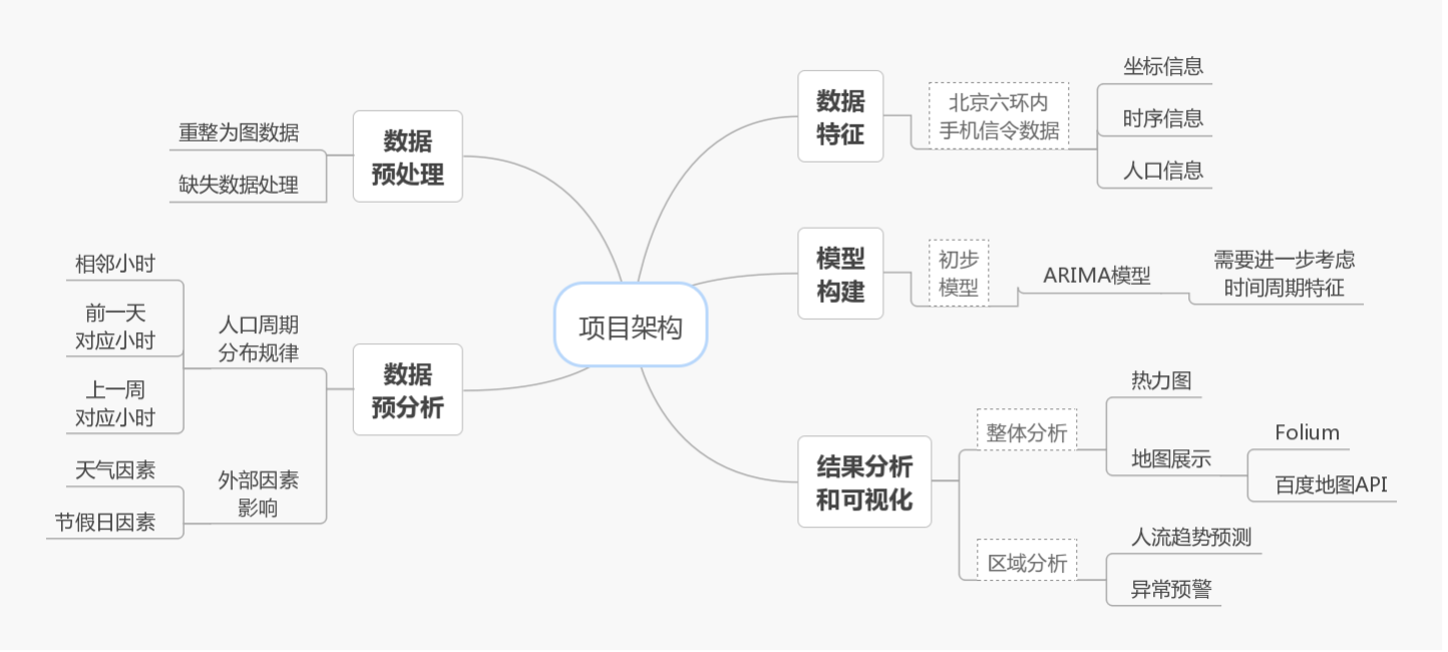
\includegraphics[width=\textwidth]{timeline.png}
\caption{项目架构}
\label{fig:A1}
\end{figure}
其中残差网络的架构为(图\ref{fig:A2})
\begin{figure}[ht]
\centering
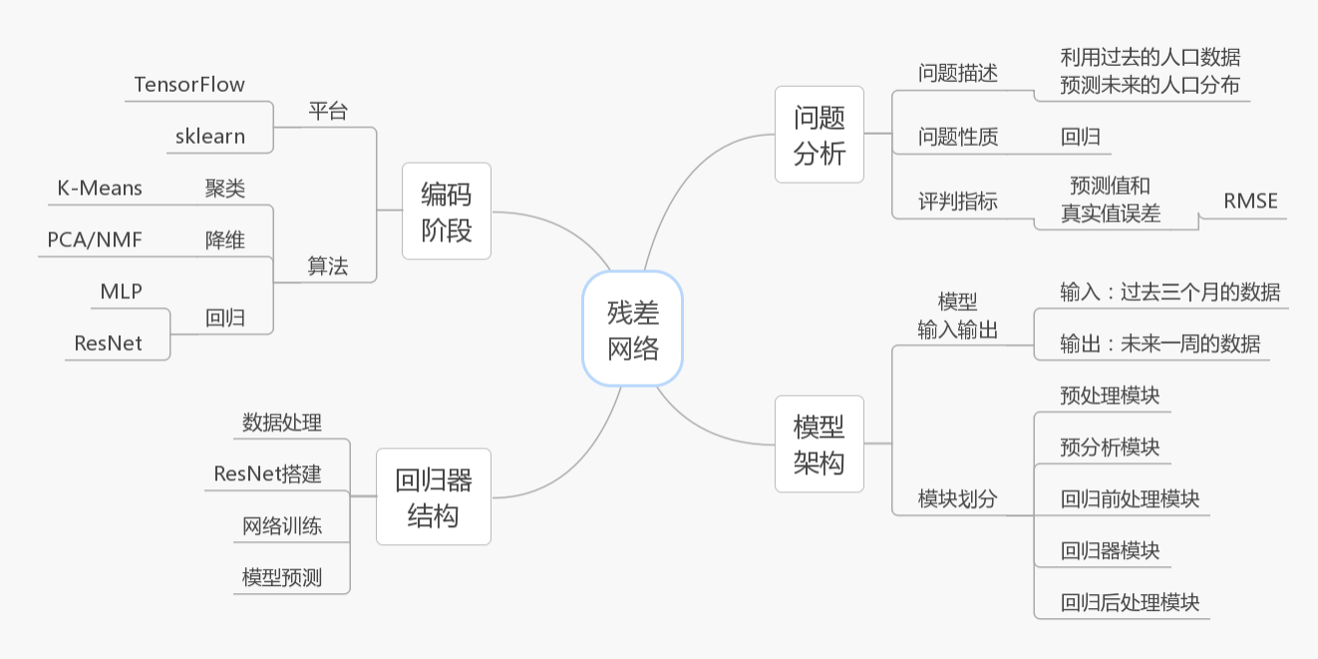
\includegraphics[width=\textwidth]{A2.png}
\caption{残差网络}
\label{fig:A2}
\end{figure}